\pagebreak
\subsection{5a \& 5b}
\begin{figure}[H]
    \centering
    \begin{subfigure}{0.5\textwidth}
        \centering
        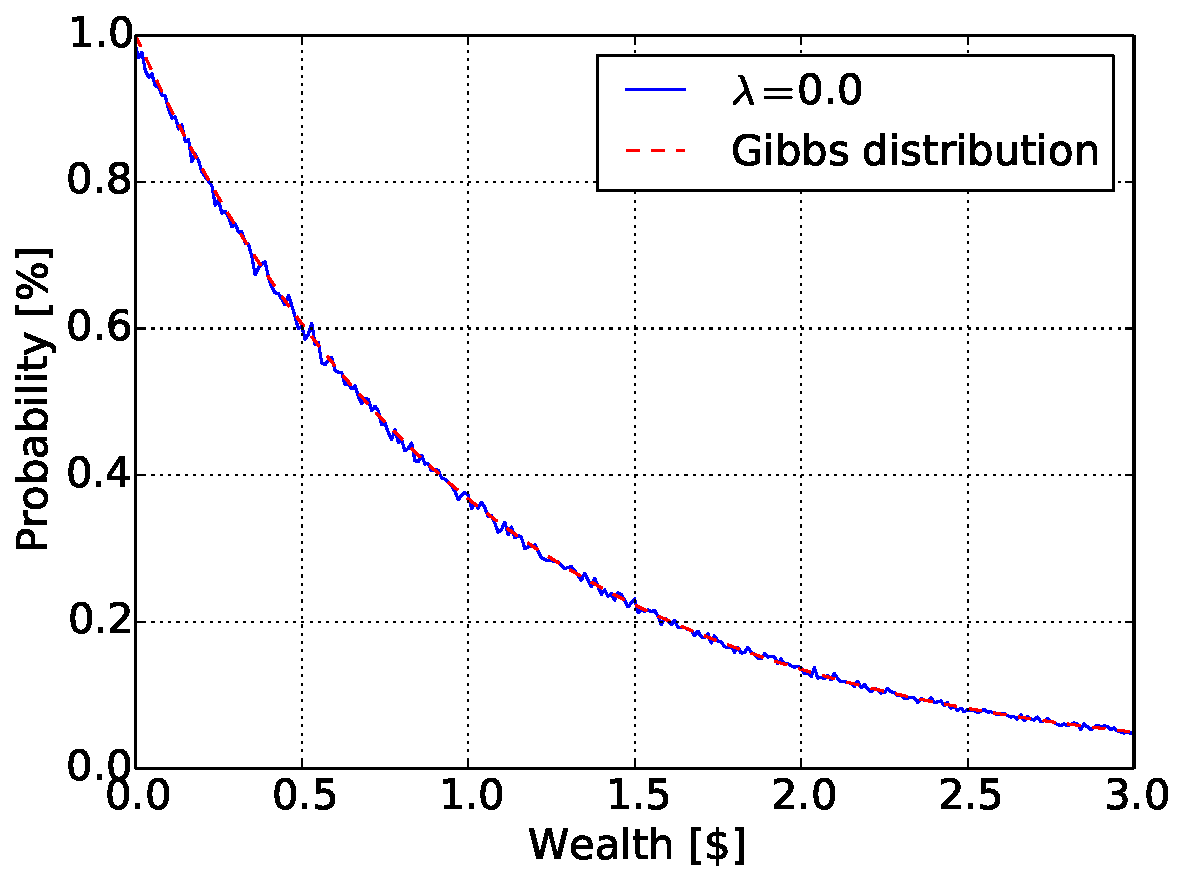
\includegraphics[width=\linewidth]{result/bilder/5a-correct}
        \caption{}
    \end{subfigure}%
    ~ 
    \begin{subfigure}{0.5\textwidth}
        \centering
        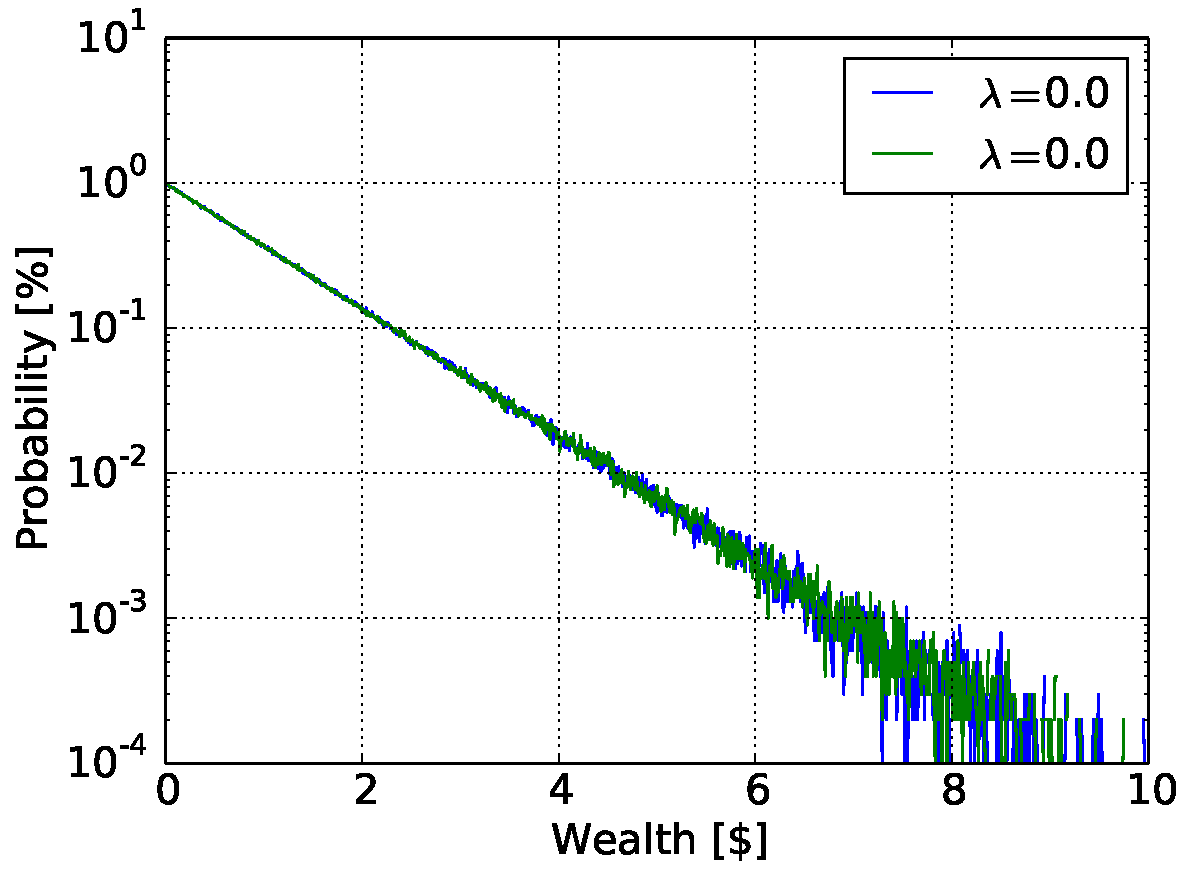
\includegraphics[width=\linewidth]{result/bilder/5b-correct}
        \caption{}
    \end{subfigure}
    \caption{a) Shows how E behaves around $T_C$ b) Shows how |M| develops near $T_C$.}
    \label{fig:5a-b}
\end{figure}




























\pagebreak
\subsection{5c}
\begin{figure}[H]
    \centering
    \begin{subfigure}{0.5\textwidth}
        \centering
        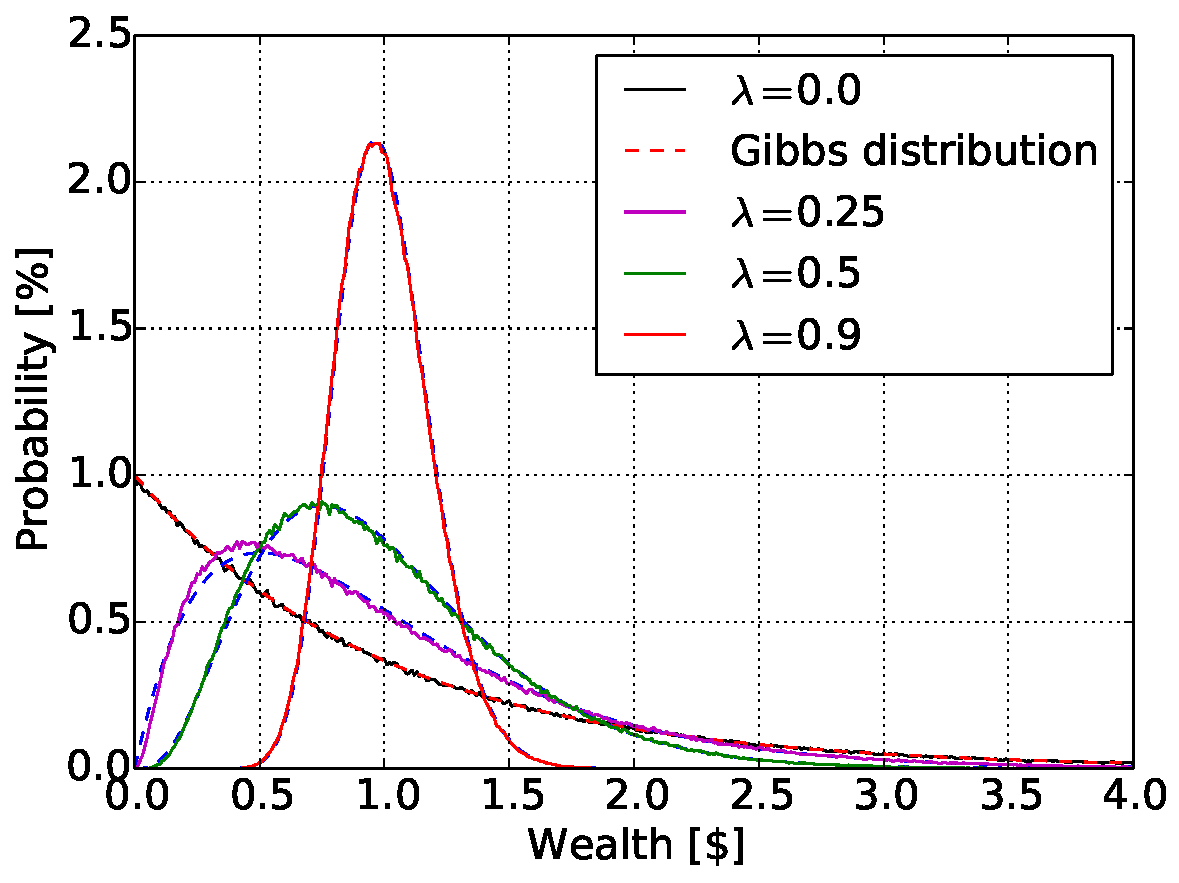
\includegraphics[width=\linewidth]{result/bilder/5c}
        \caption{}
    \end{subfigure}%
    ~ 
    \begin{subfigure}{0.5\textwidth}
        \centering
        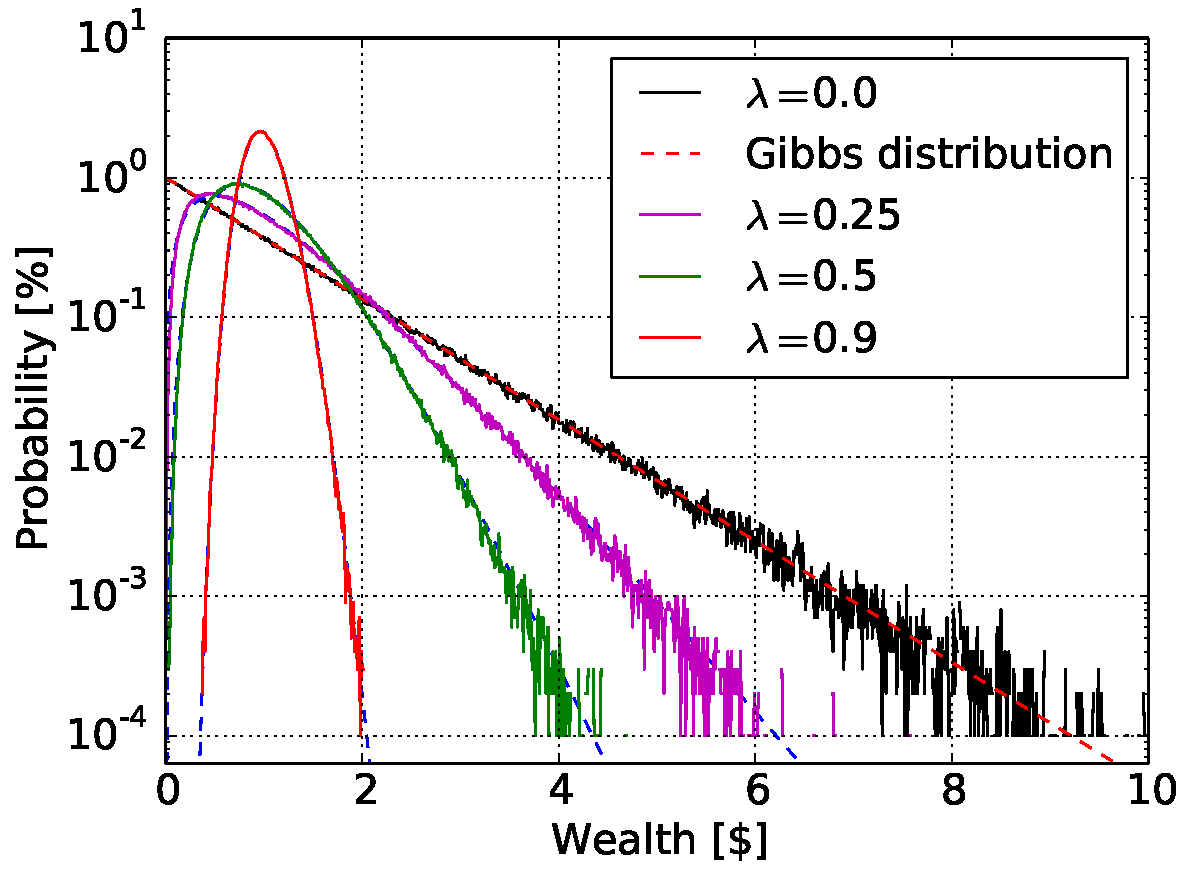
\includegraphics[width=\linewidth]{result/bilder/5c-log}
        \caption{}
    \end{subfigure}
    \caption{a) Shows how E behaves around $T_C$ b) Shows how |M| develops near $T_C$.}
    \label{fig:5c}
\end{figure}




























\pagebreak
\subsection{5d}
\begin{figure}[H]
    \centering
    \begin{subfigure}{0.5\textwidth}
        \centering
        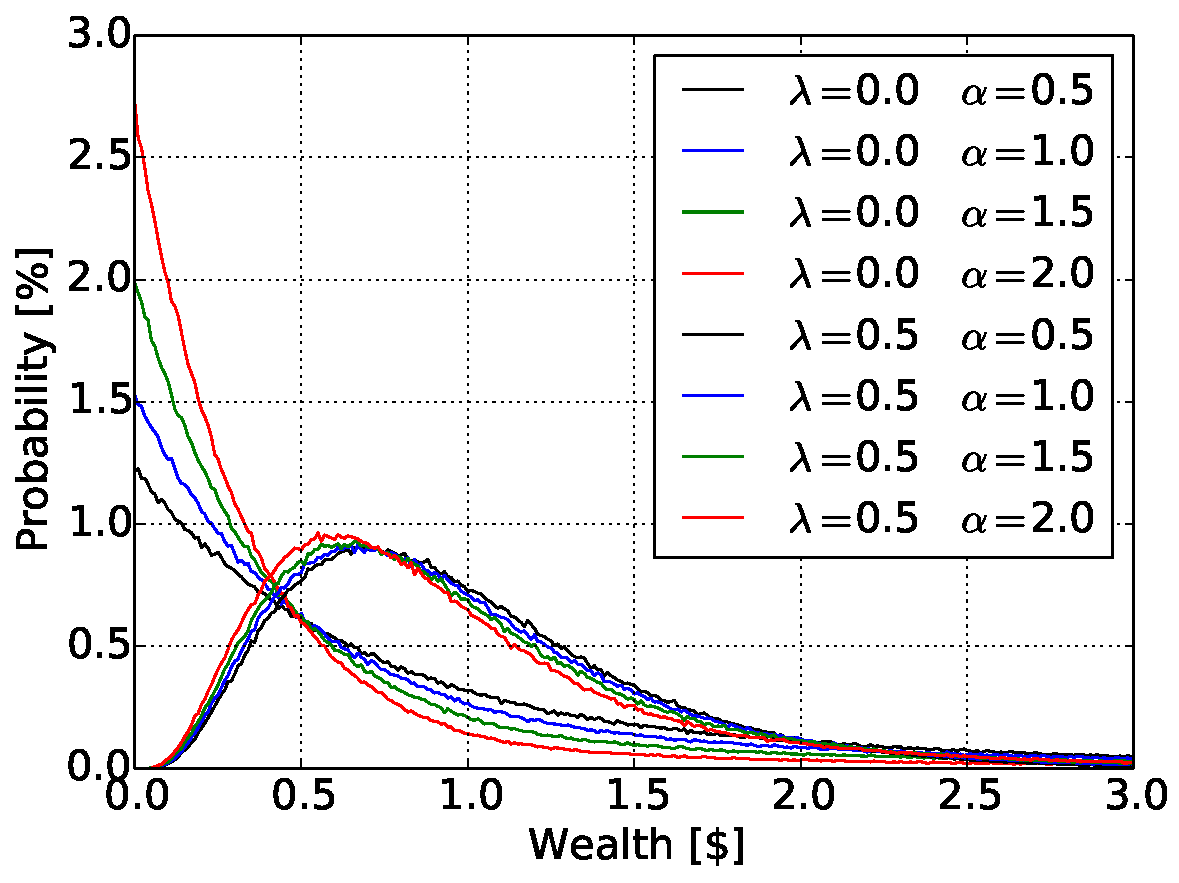
\includegraphics[width=\linewidth]{result/bilder/5d-0050}
        \caption{}
    \end{subfigure}%
    ~ 
    \begin{subfigure}{0.5\textwidth}
        \centering
        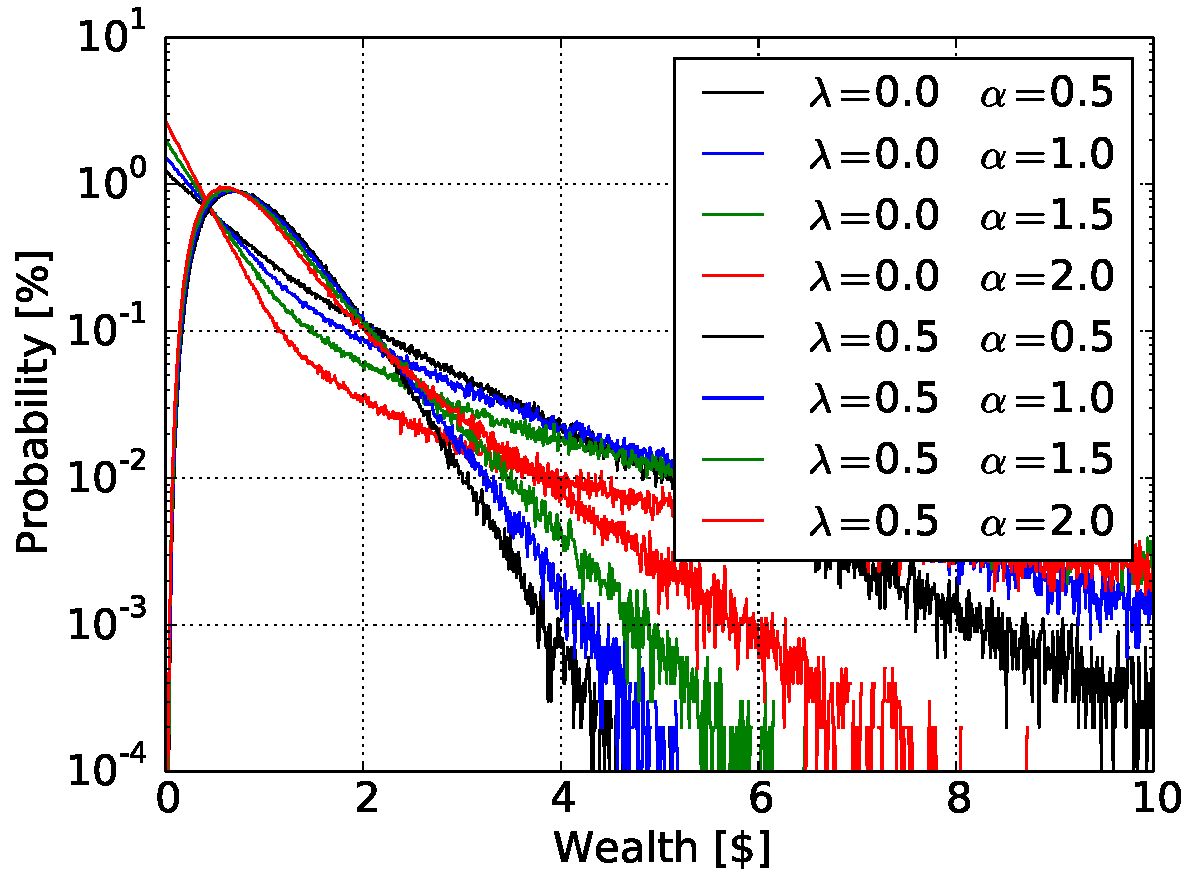
\includegraphics[width=\linewidth]{result/bilder/5d-0050-log}
        \caption{}
    \end{subfigure}
    \caption{a) Shows how E behaves around $T_C$ b) Shows how |M| develops near $T_C$.}
    \label{fig:5d-0050}
\end{figure}



\begin{figure}[H]
    \centering
    \begin{subfigure}{0.5\textwidth}
        \centering
        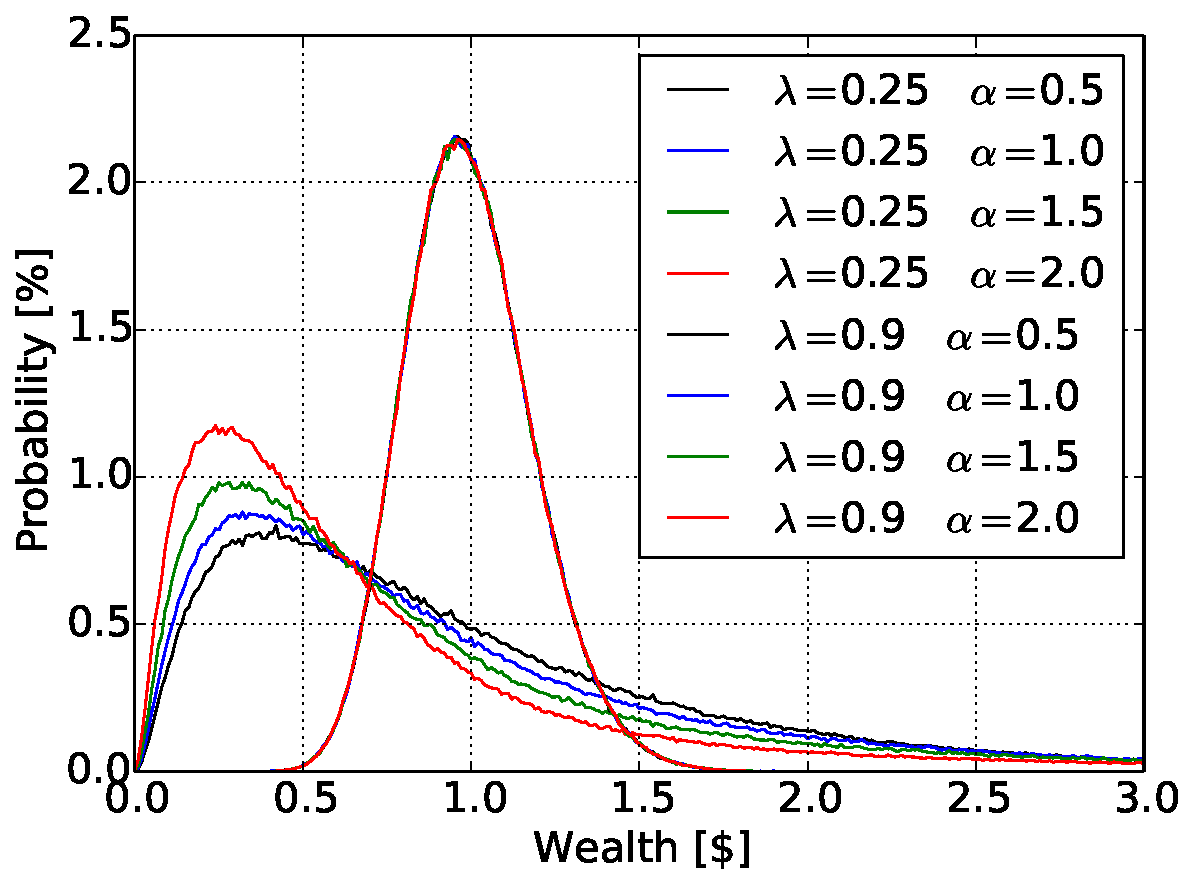
\includegraphics[width=\linewidth]{result/bilder/5d-2590}
        \caption{}
    \end{subfigure}%
    ~ 
    \begin{subfigure}{0.5\textwidth}
        \centering
        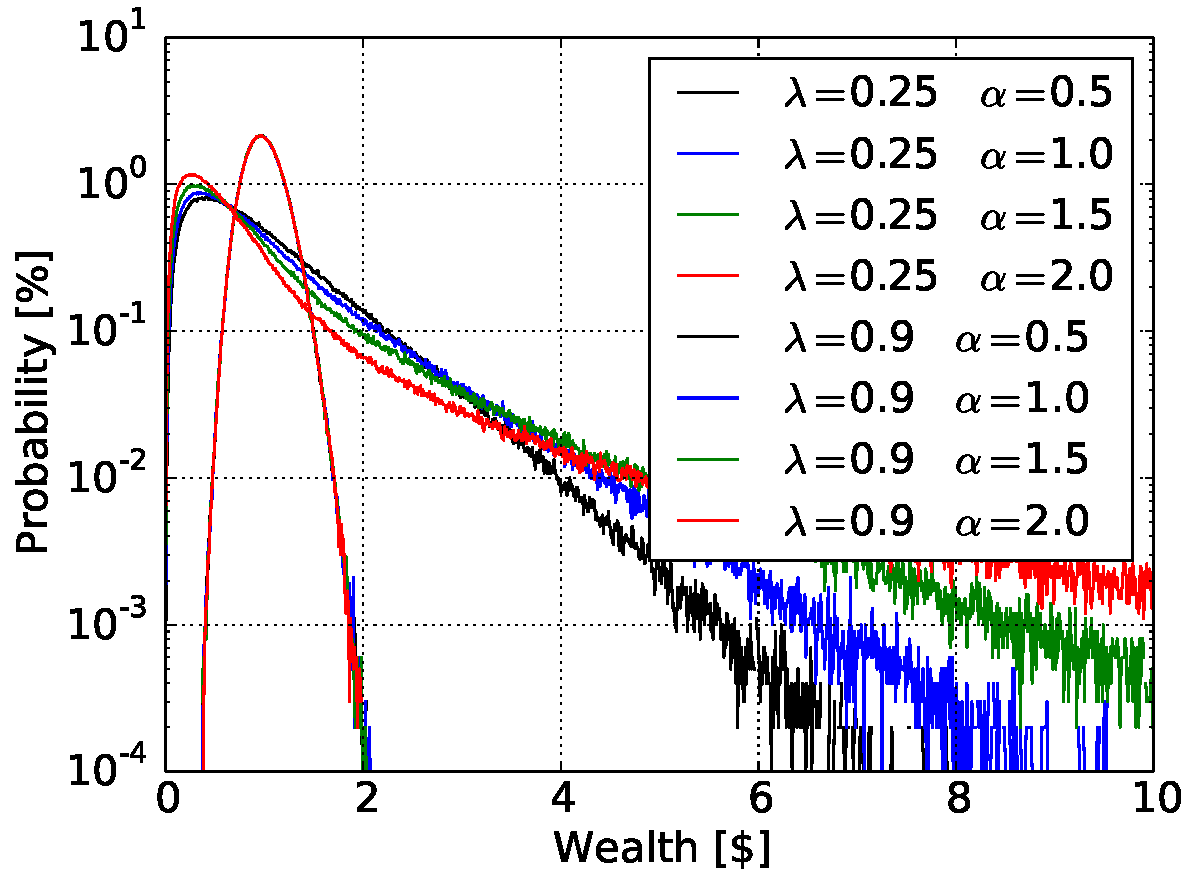
\includegraphics[width=\linewidth]{result/bilder/5d-2590-log}
        \caption{}
    \end{subfigure}
    \caption{a) Shows how E behaves around $T_C$ b) Shows how |M| develops near $T_C$.}
    \label{fig:5d-2590}
\end{figure}



\begin{figure}[H]
    \centering
    \begin{subfigure}{0.5\textwidth}
        \centering
        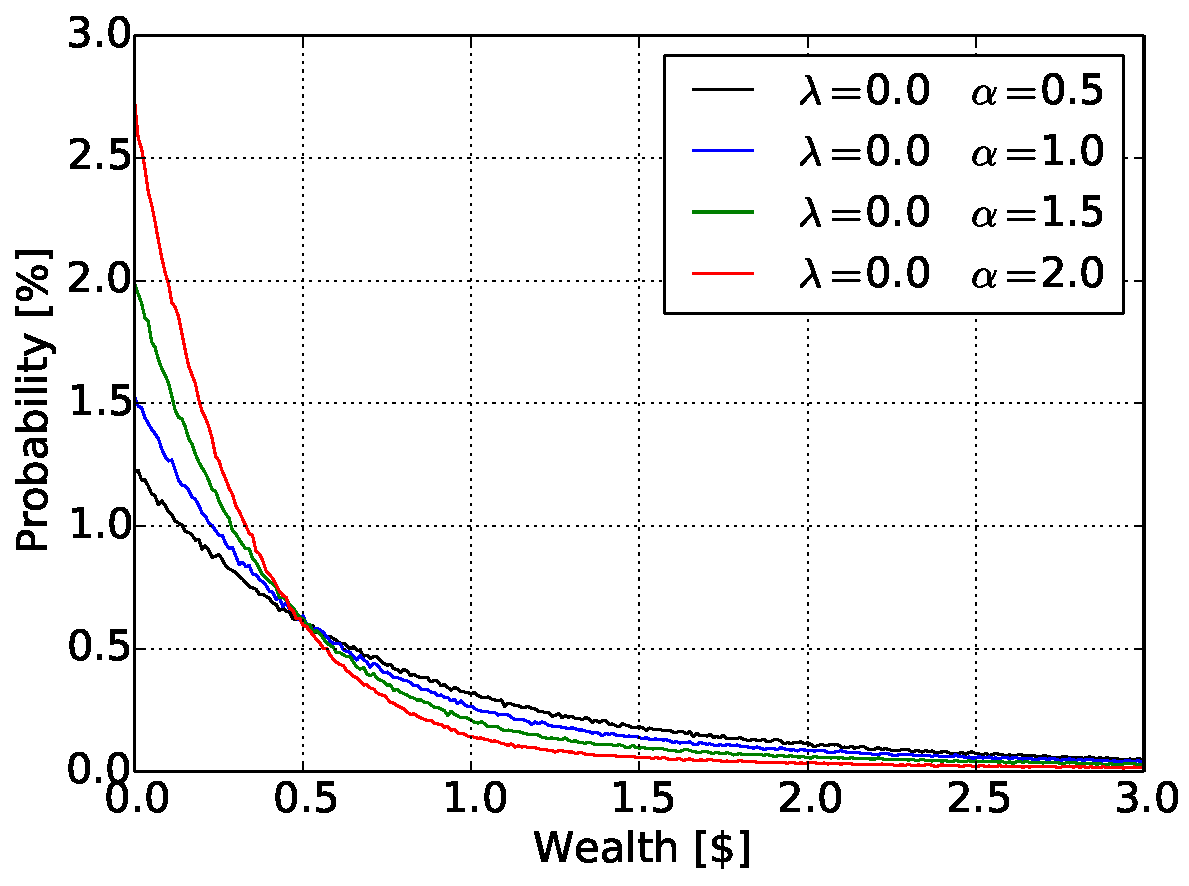
\includegraphics[width=\linewidth]{result/bilder/5d-00}
        \caption{}
    \end{subfigure}%
    ~ 
    \begin{subfigure}{0.5\textwidth}
        \centering
        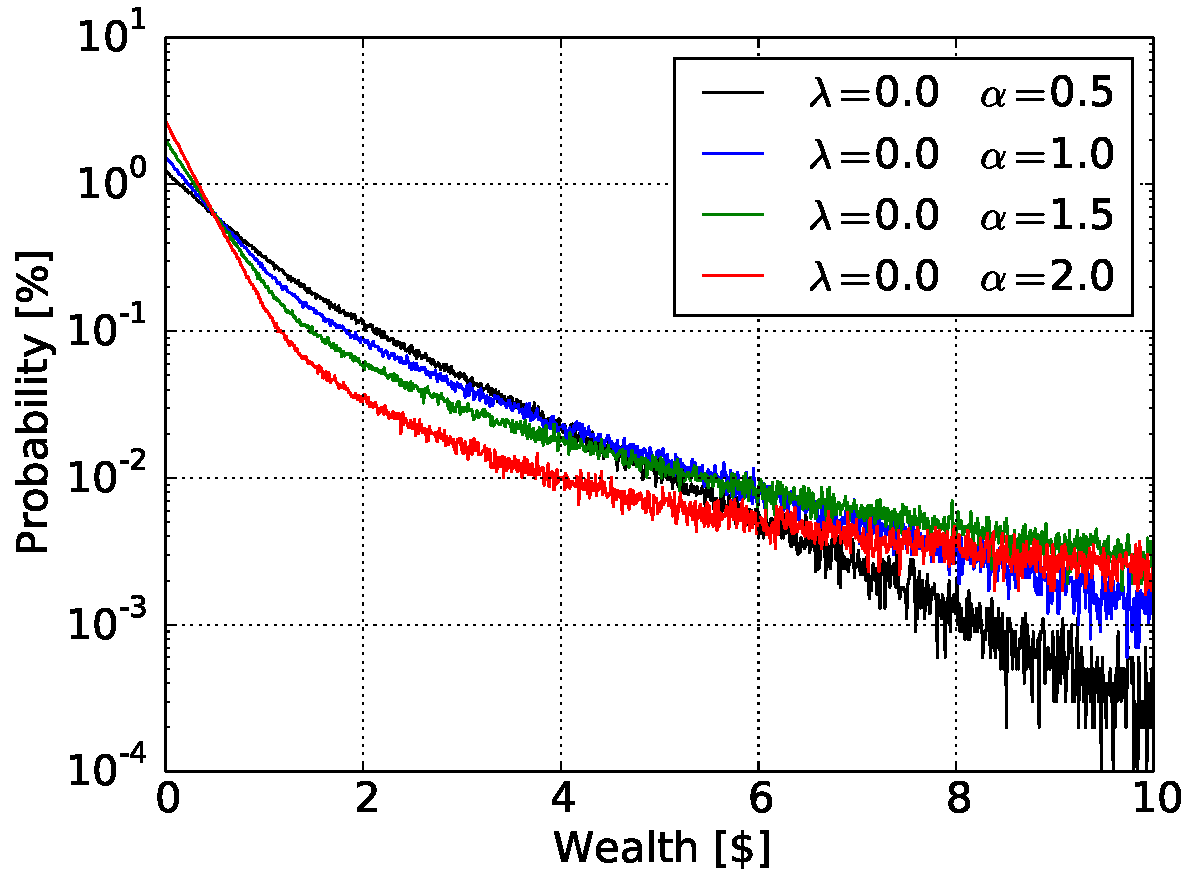
\includegraphics[width=\linewidth]{result/bilder/5d-00-log}
        \caption{}
    \end{subfigure}
    \caption{a) Shows how E behaves around $T_C$ b) Shows how |M| develops near $T_C$.}
    \label{fig:5d-00}
\end{figure}



\begin{figure}[H]
    \centering
    \begin{subfigure}{0.5\textwidth}
        \centering
        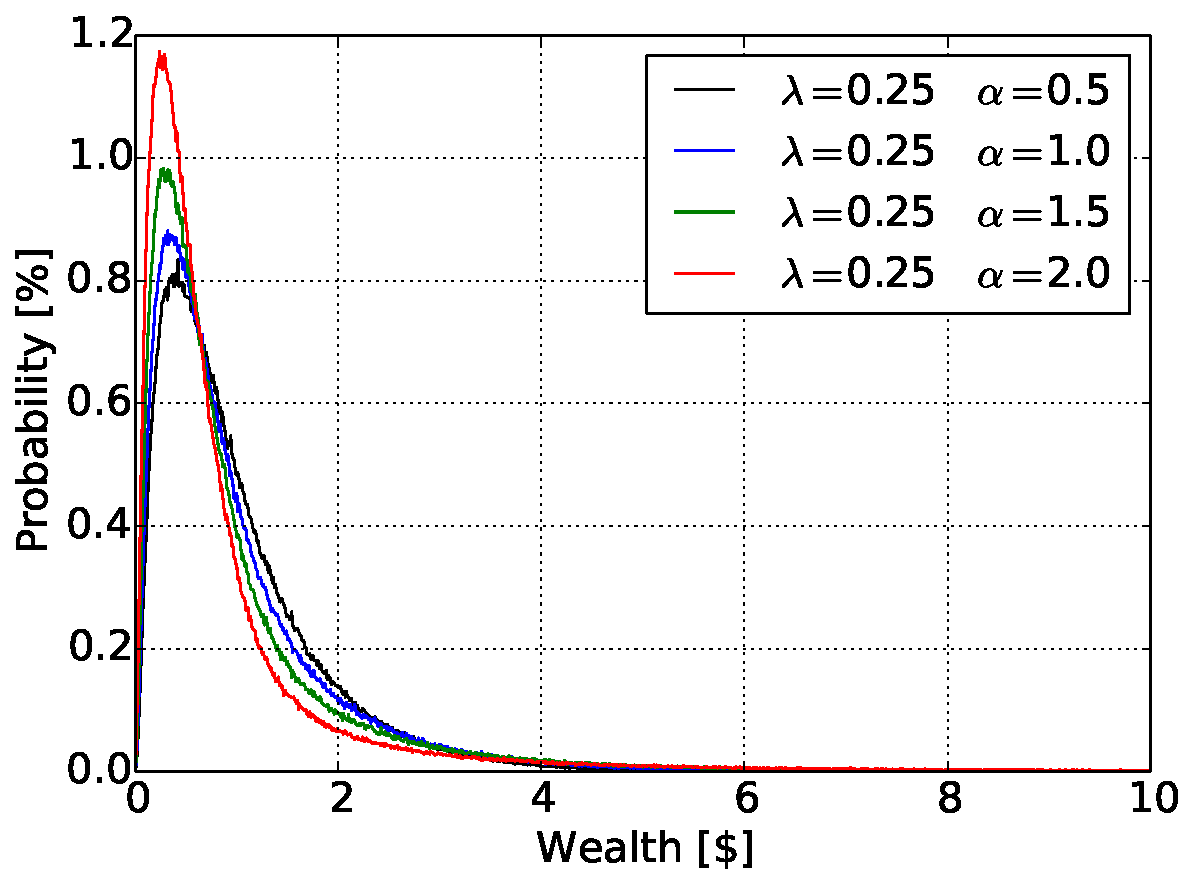
\includegraphics[width=\linewidth]{result/bilder/5d-25}
        \caption{}
    \end{subfigure}%
    ~ 
    \begin{subfigure}{0.5\textwidth}
        \centering
        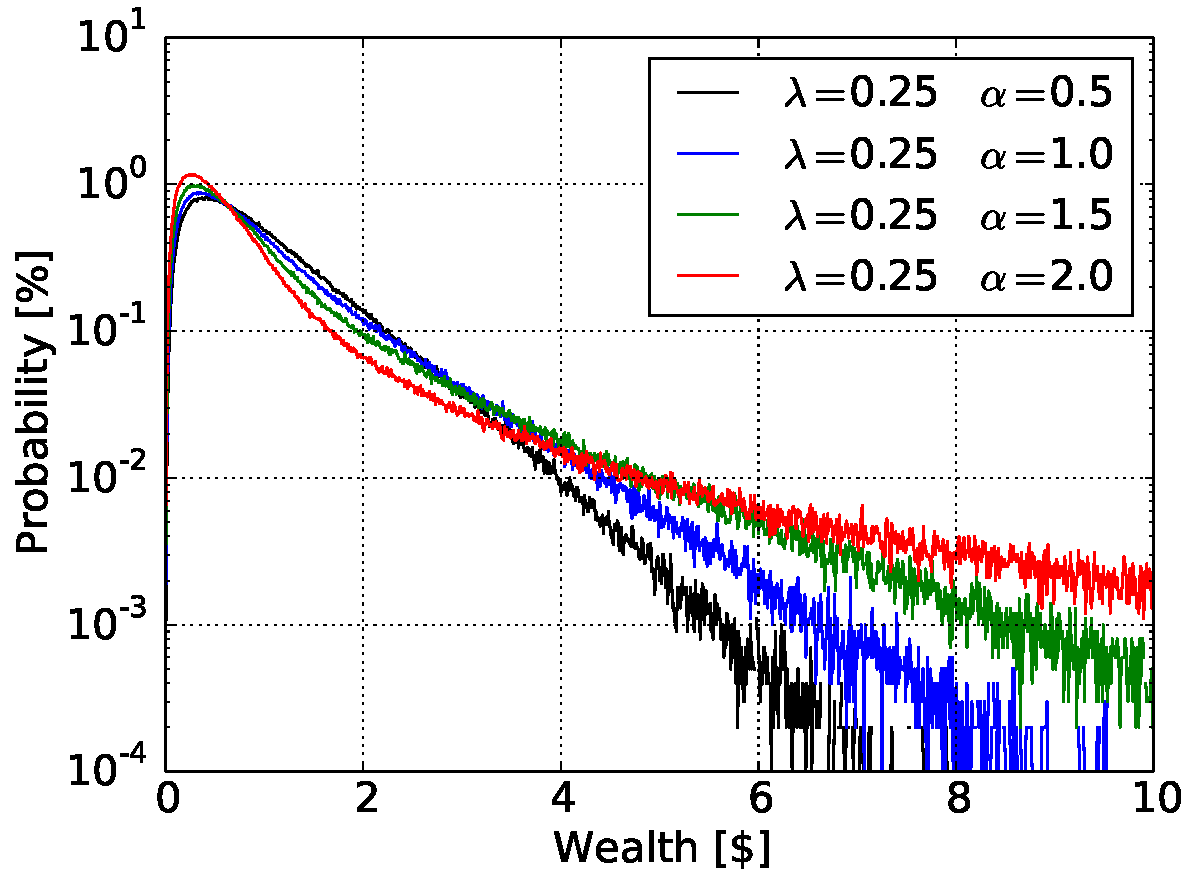
\includegraphics[width=\linewidth]{result/bilder/5d-25-log}
        \caption{}
    \end{subfigure}
    \caption{a) Shows how E behaves around $T_C$ b) Shows how |M| develops near $T_C$.}
    \label{fig:5d-25}
\end{figure}




\begin{figure}[H]
    \centering
    \begin{subfigure}{0.5\textwidth}
        \centering
        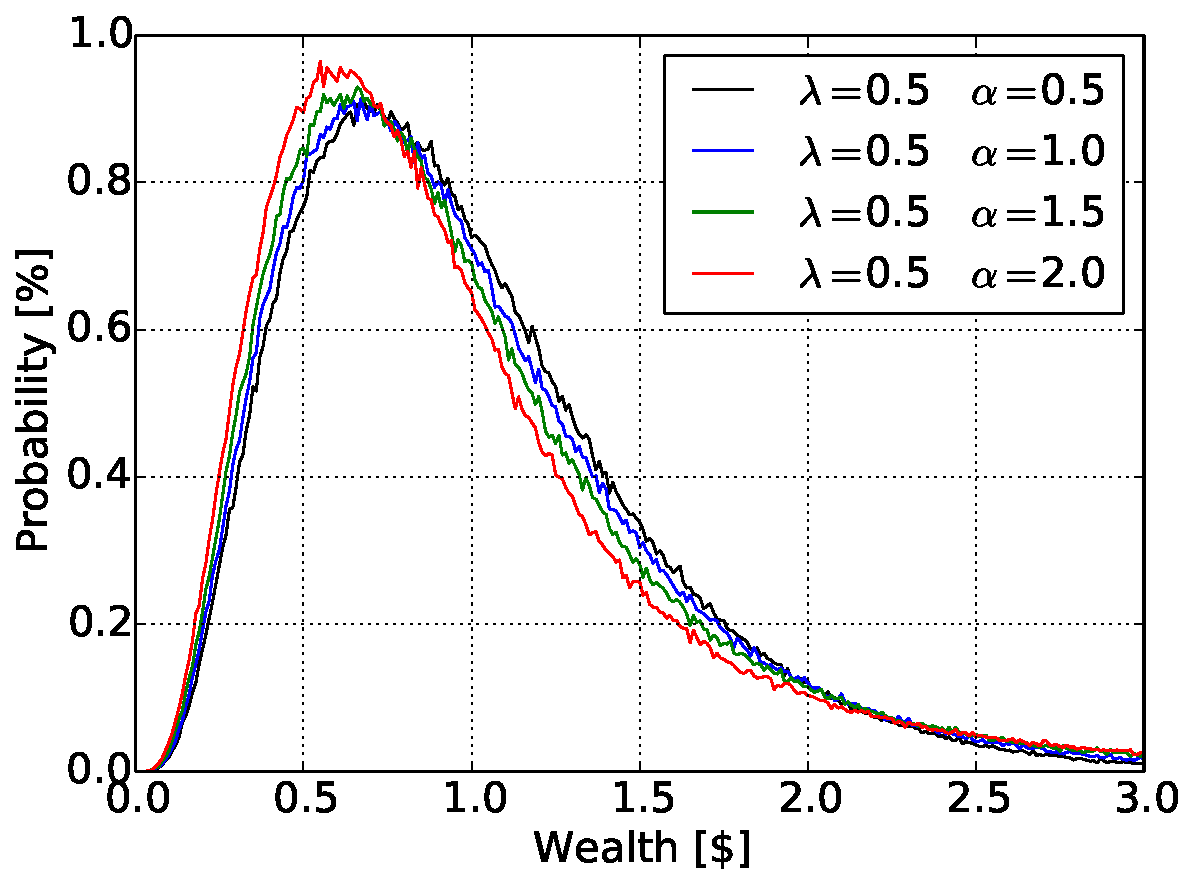
\includegraphics[width=\linewidth]{result/bilder/5d-50}
        \caption{}
    \end{subfigure}%
    ~ 
    \begin{subfigure}{0.5\textwidth}
        \centering
        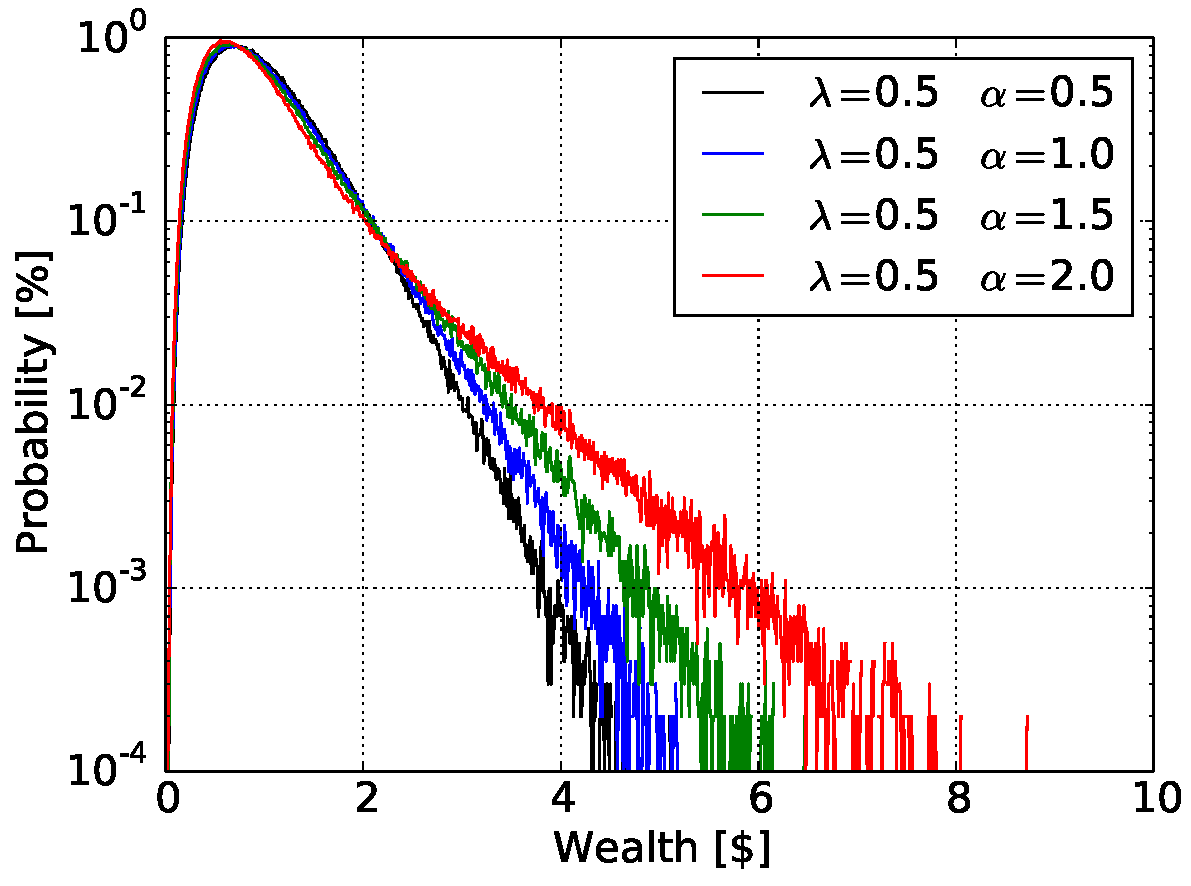
\includegraphics[width=\linewidth]{result/bilder/5d-50-log}
        \caption{}
    \end{subfigure}
    \caption{a) Shows how E behaves around $T_C$ b) Shows how |M| develops near $T_C$.}
    \label{fig:5d-50}
\end{figure}



\begin{figure}[H]
    \centering
    \begin{subfigure}{0.5\textwidth}
        \centering
        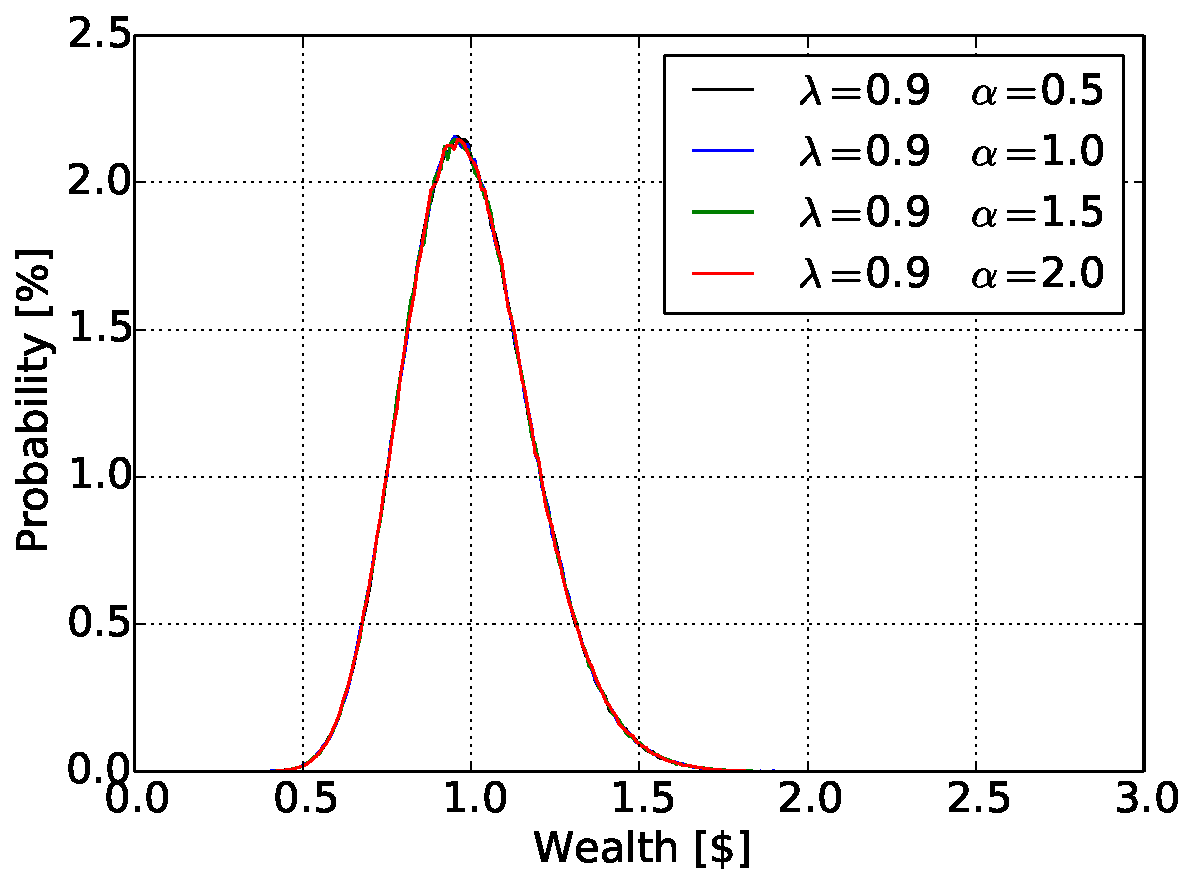
\includegraphics[width=\linewidth]{result/bilder/5d-90}
        \caption{}
    \end{subfigure}%
    ~ 
    \begin{subfigure}{0.5\textwidth}
        \centering
        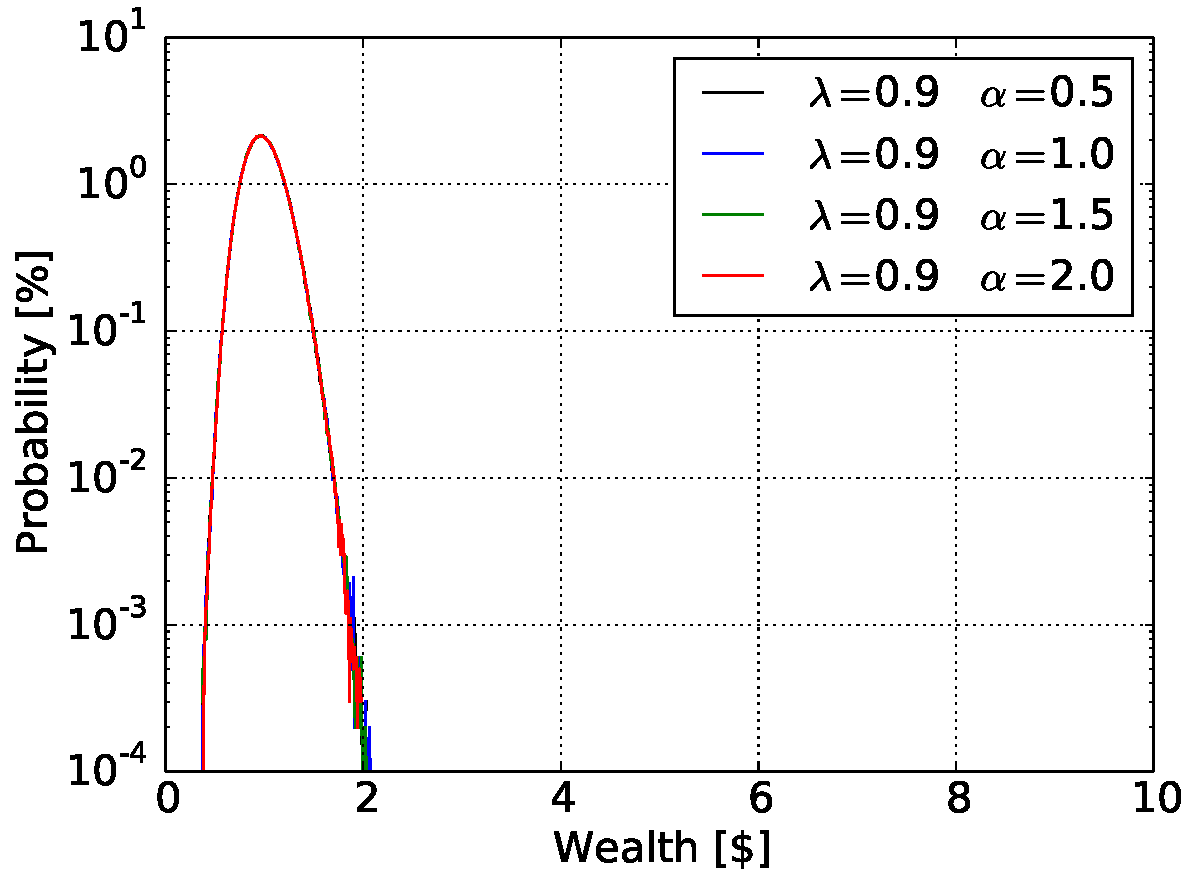
\includegraphics[width=\linewidth]{result/bilder/5d-90-log}
        \caption{}
    \end{subfigure}
    \caption{a) Shows how E behaves around $T_C$ b) Shows how |M| develops near $T_C$.}
    \label{fig:5d-90}
\end{figure}
























\pagebreak
\subsection{5e}
\begin{figure}[H]
    \centering
    \begin{subfigure}{0.5\textwidth}
        \centering
        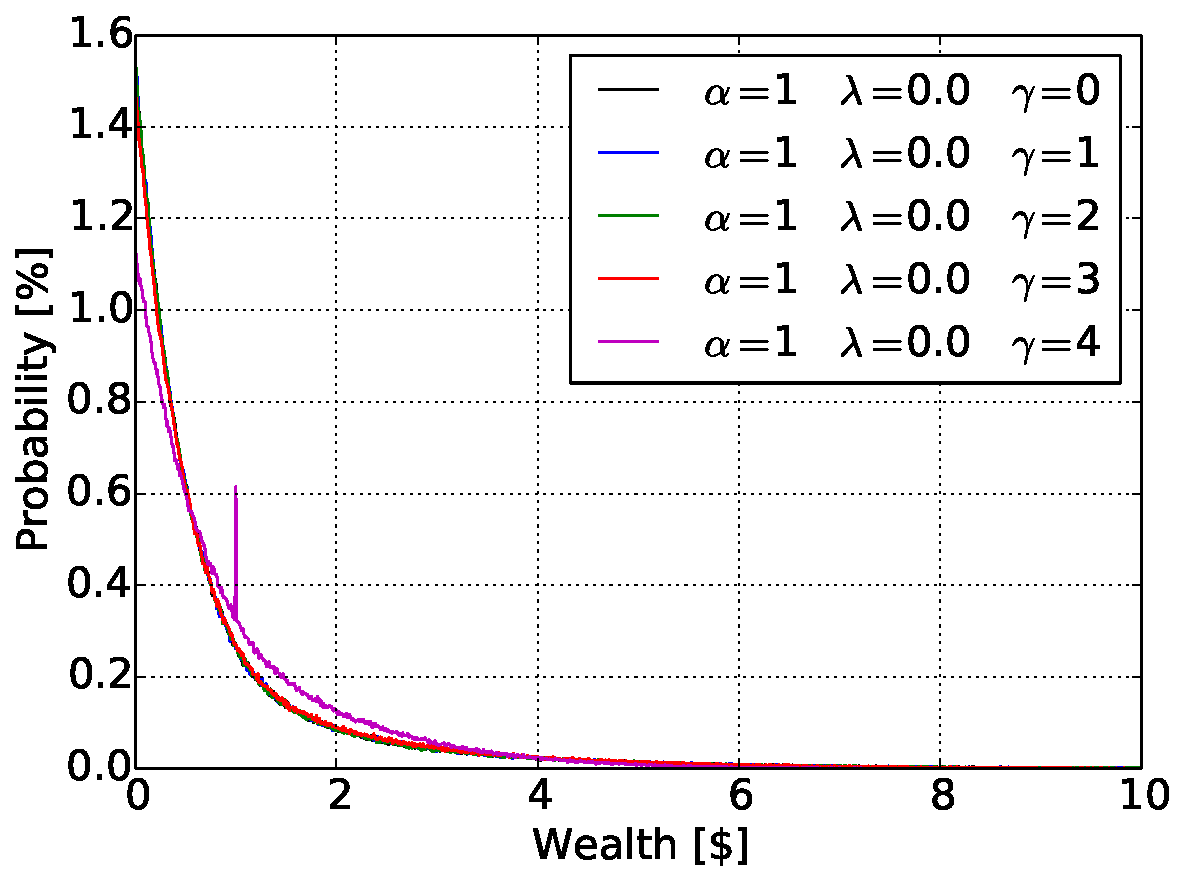
\includegraphics[width=\linewidth]{result/bilder/5e-1-00}
        \caption{}
    \end{subfigure}%
    ~ 
    \begin{subfigure}{0.5\textwidth}
        \centering
        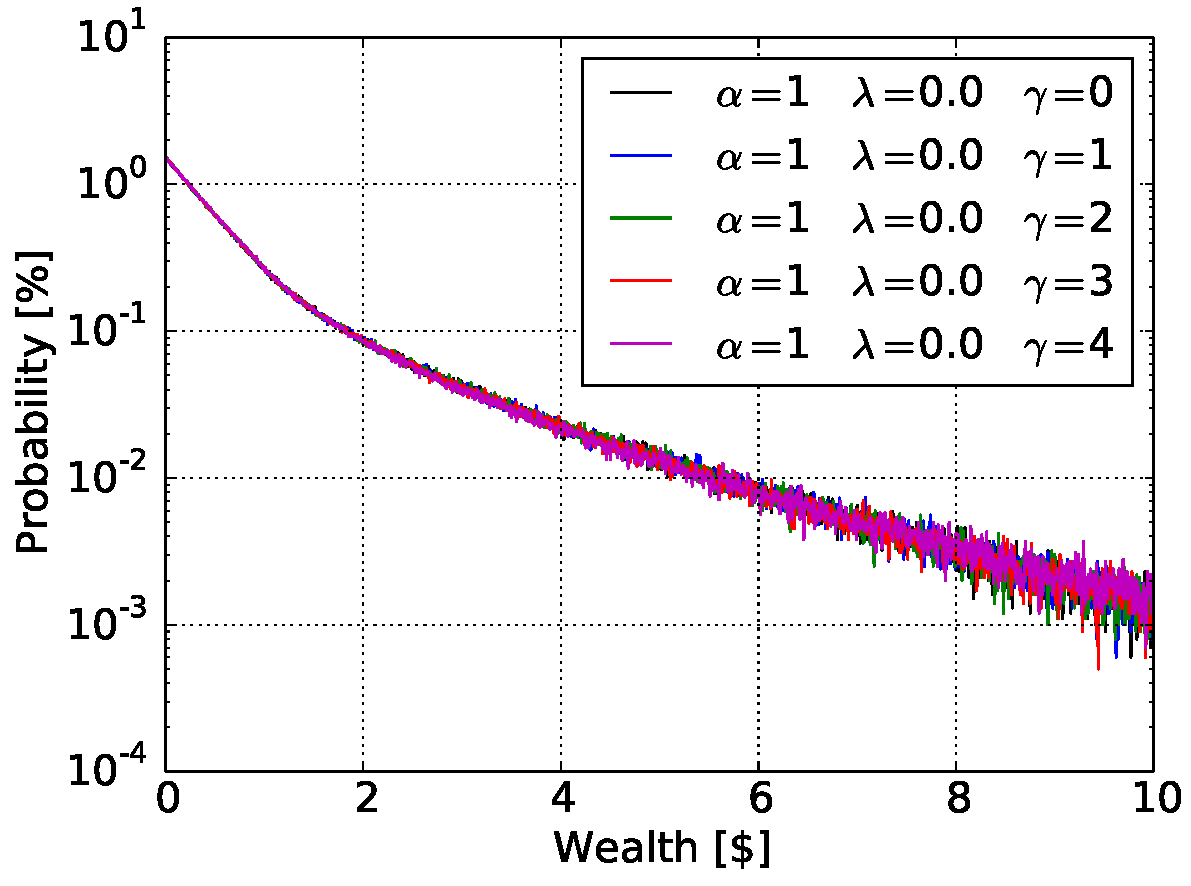
\includegraphics[width=\linewidth]{result/bilder/5e-1-00-log}
        \caption{}
    \end{subfigure}
    \caption{a) Shows how E behaves around $T_C$ b) Shows how |M| develops near $T_C$.}
    \label{fig:5e-1-00}
\end{figure}



\begin{figure}[H]
    \centering
    \begin{subfigure}{0.5\textwidth}
        \centering
        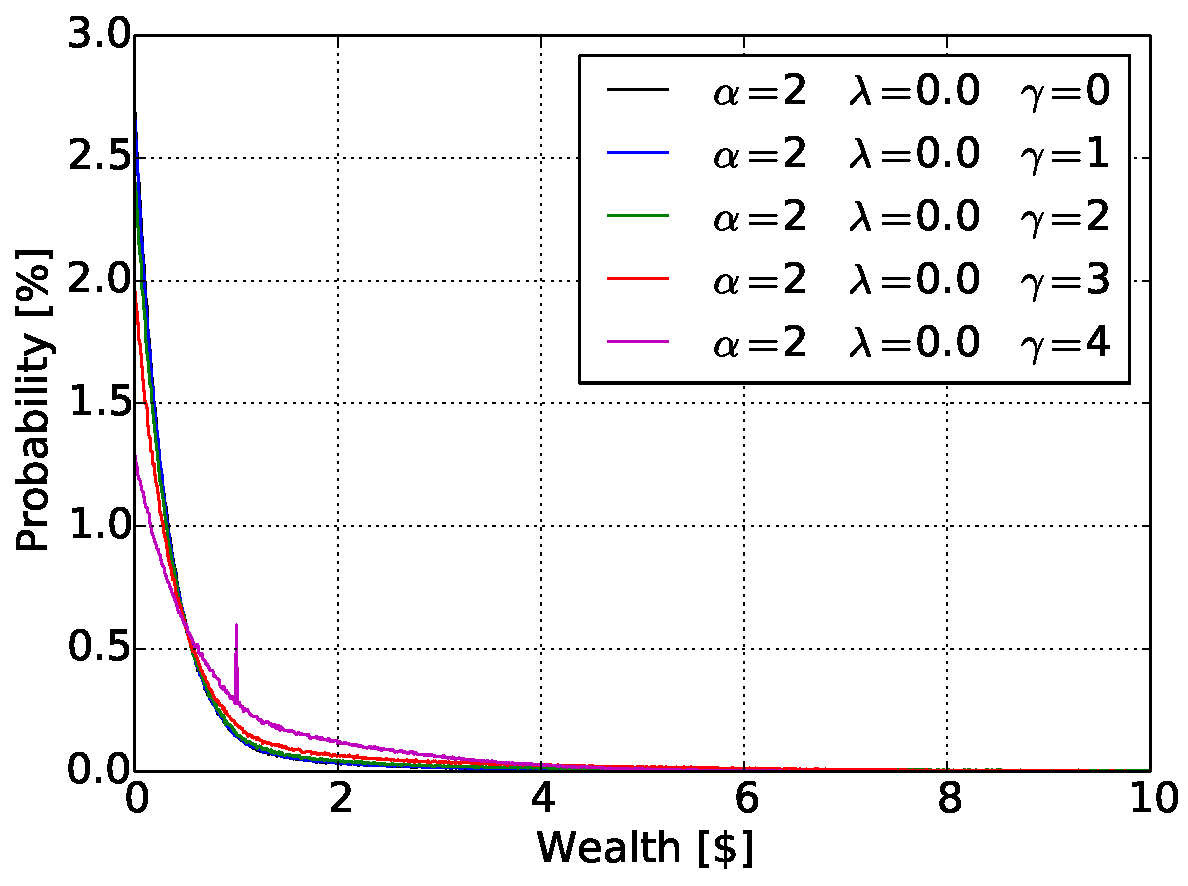
\includegraphics[width=\linewidth]{result/bilder/5e-2-00}
        \caption{}
    \end{subfigure}%
    ~ 
    \begin{subfigure}{0.5\textwidth}
        \centering
        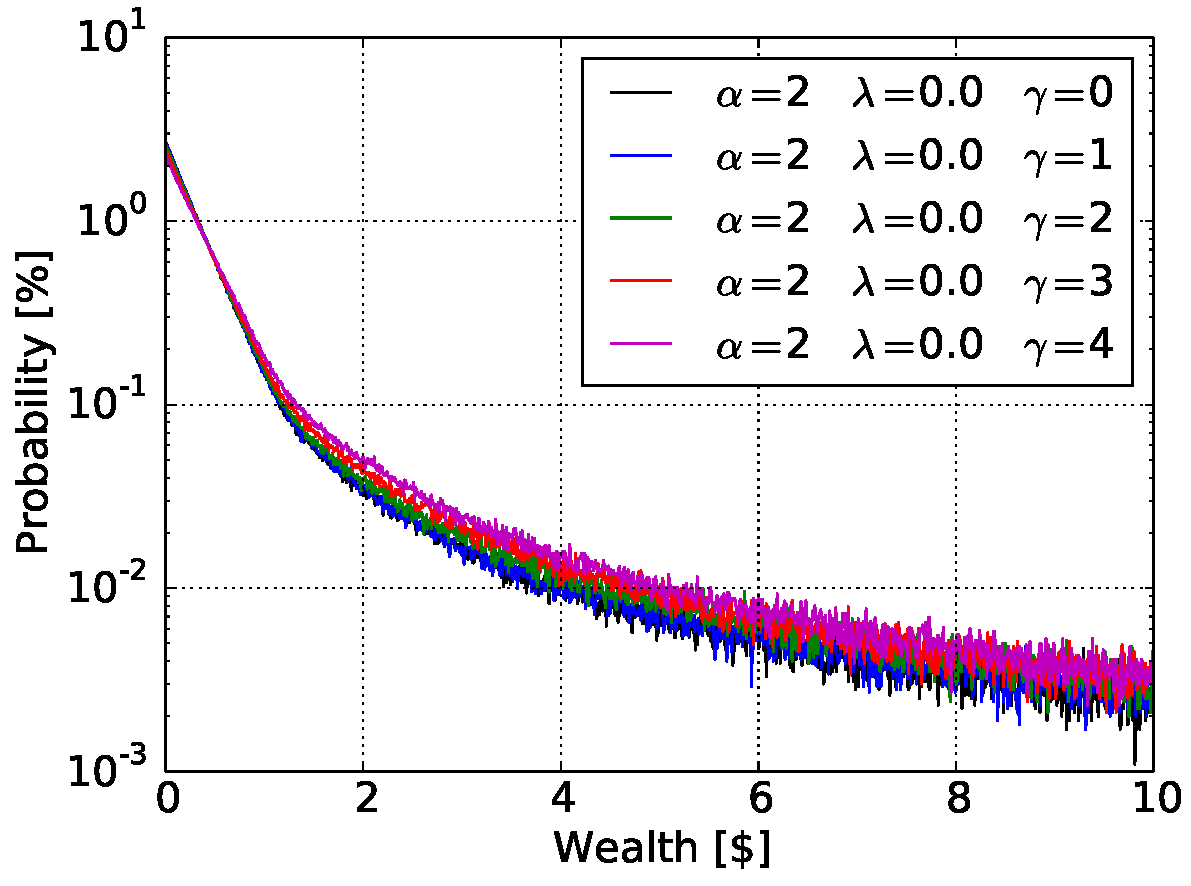
\includegraphics[width=\linewidth]{result/bilder/5e-2-00-log}
        \caption{}
    \end{subfigure}
    \caption{a) Shows how E behaves around $T_C$ b) Shows how |M| develops near $T_C$.}
    \label{fig:5e-2-00}
\end{figure}














\begin{figure}[H]
    \centering
    \begin{subfigure}{0.5\textwidth}
        \centering
        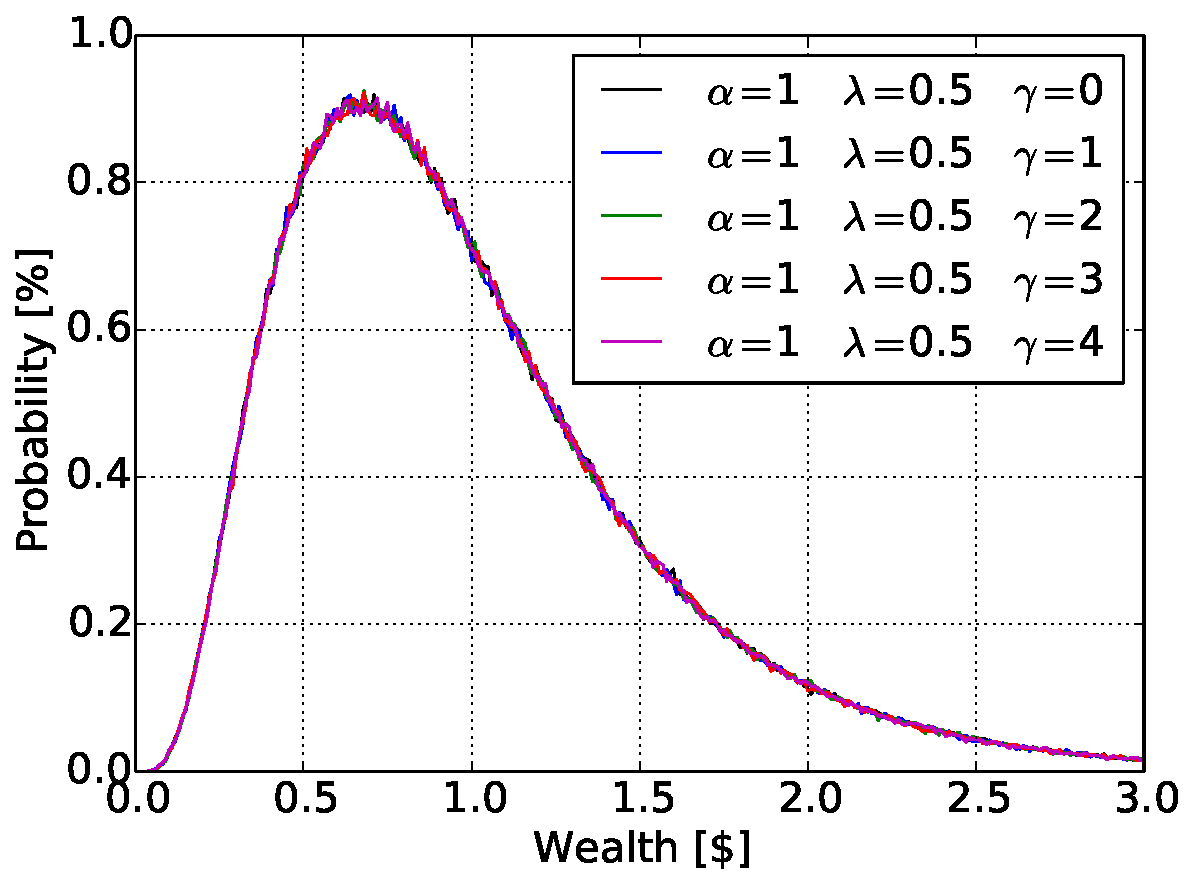
\includegraphics[width=\linewidth]{result/bilder/5e-1-50}
        \caption{}
    \end{subfigure}%
    ~ 
    \begin{subfigure}{0.5\textwidth}
        \centering
        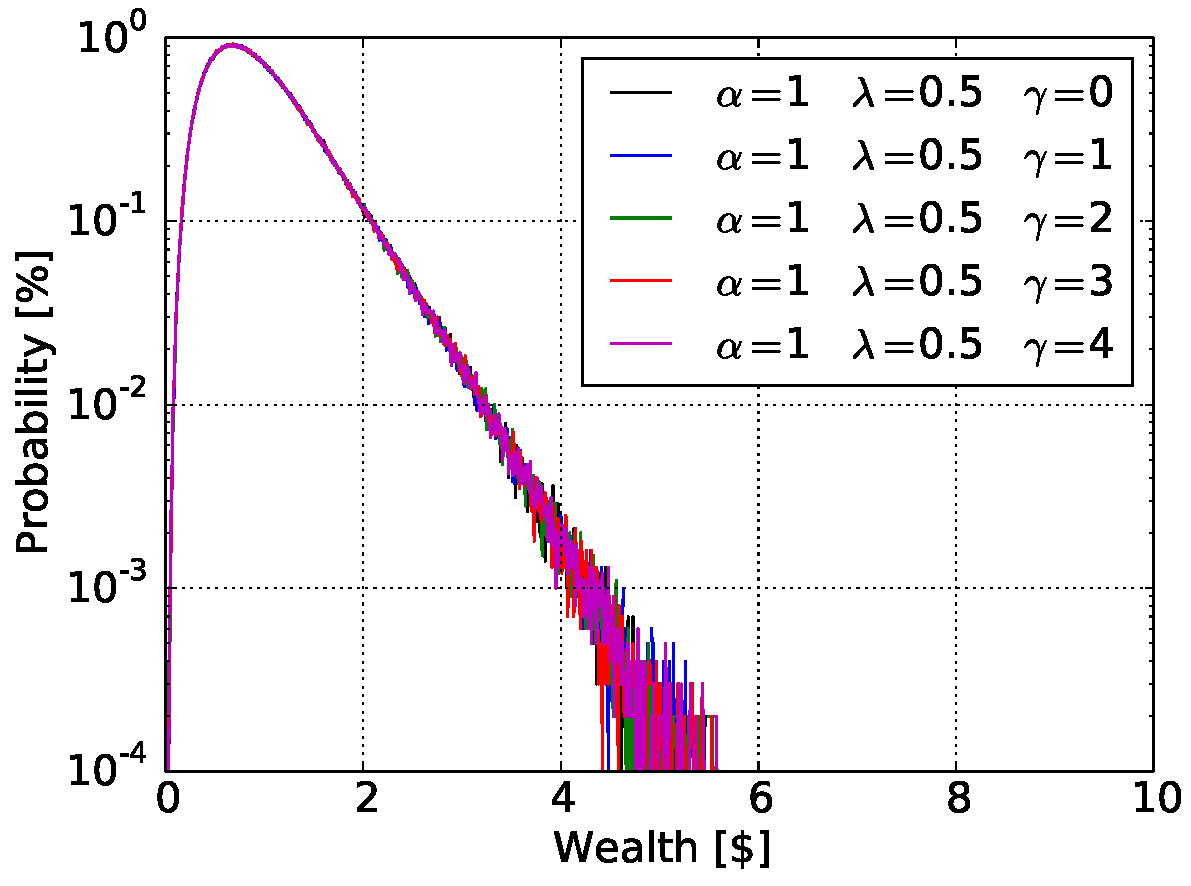
\includegraphics[width=\linewidth]{result/bilder/5e-1-50-log}
        \caption{}
    \end{subfigure}
    \caption{a) Shows how E behaves around $T_C$ b) Shows how |M| develops near $T_C$.}
    \label{fig:5e-1-50}
\end{figure}



\begin{figure}[H]
    \centering
    \begin{subfigure}{0.5\textwidth}
        \centering
        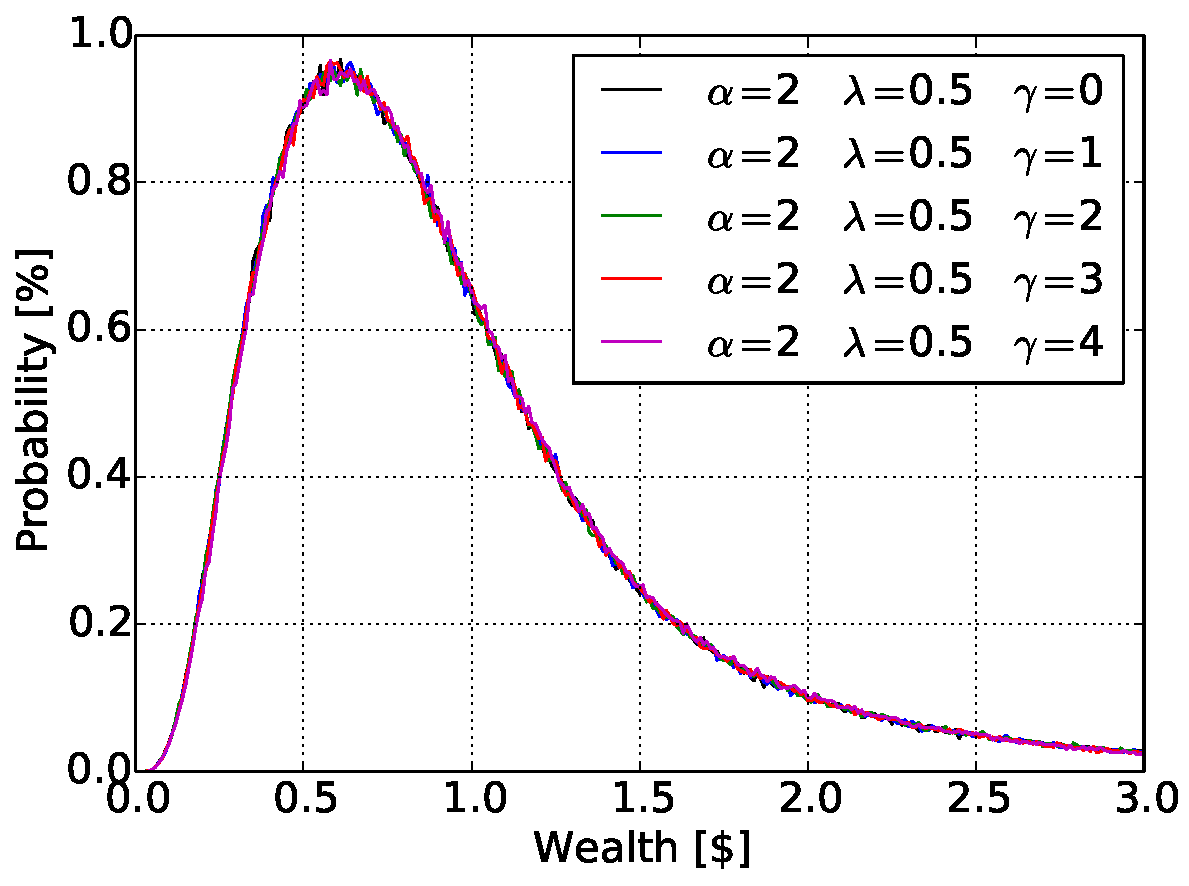
\includegraphics[width=\linewidth]{result/bilder/5e-2-50}
        \caption{}
    \end{subfigure}%
    ~ 
    \begin{subfigure}{0.5\textwidth}
        \centering
        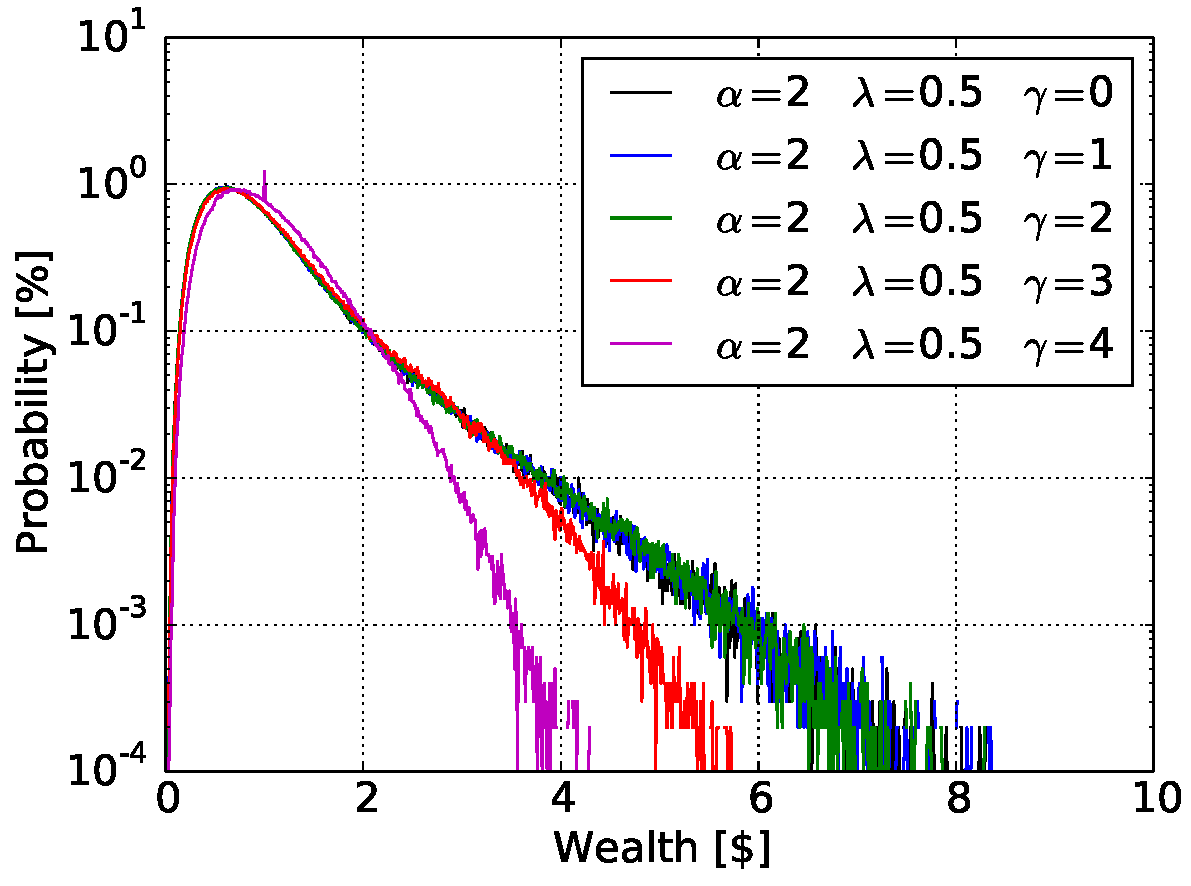
\includegraphics[width=\linewidth]{result/bilder/5e-2-50-log}
        \caption{}
    \end{subfigure}
    \caption{a) Shows how E behaves around $T_C$ b) Shows how |M| develops near $T_C$.}
    \label{fig:5e-2-50}
\end{figure}















\begin{figure}[H]
    \centering
    \begin{subfigure}{0.5\textwidth}
        \centering
        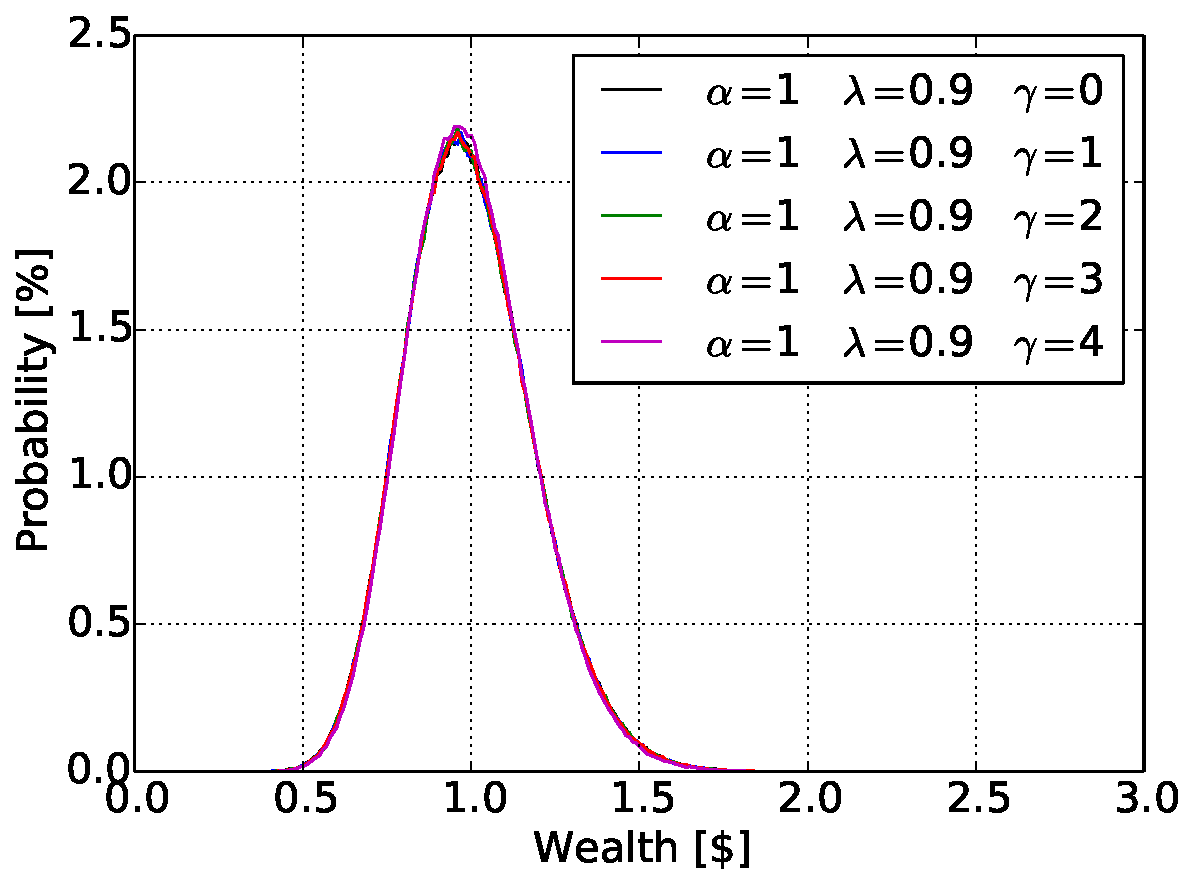
\includegraphics[width=\linewidth]{result/bilder/5e-1-90}
        \caption{}
    \end{subfigure}%
    ~ 
    \begin{subfigure}{0.5\textwidth}
        \centering
        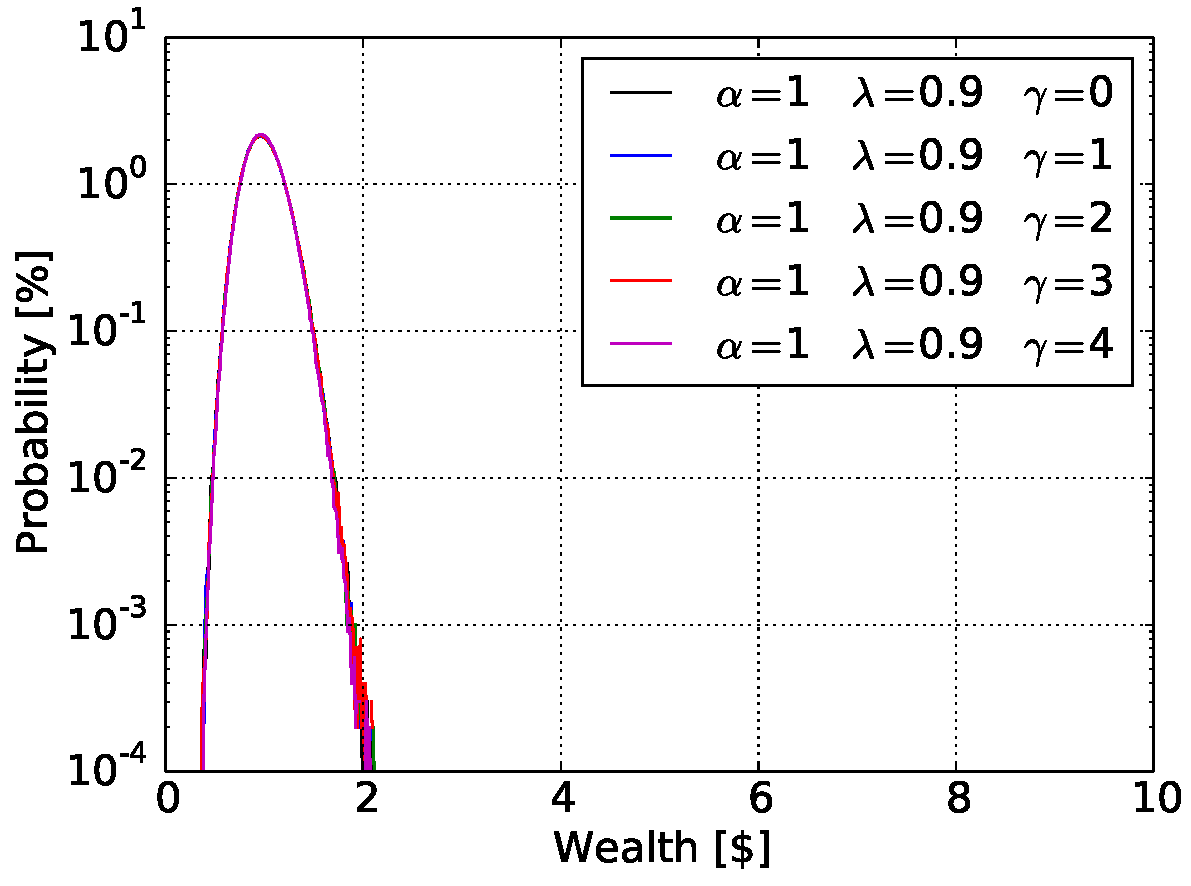
\includegraphics[width=\linewidth]{result/bilder/5e-1-90-log}
        \caption{}
    \end{subfigure}
    \caption{a) Shows how E behaves around $T_C$ b) Shows how |M| develops near $T_C$.}
    \label{fig:5e-1-90}
\end{figure}



\begin{figure}[H]
    \centering
    \begin{subfigure}{0.5\textwidth}
        \centering
        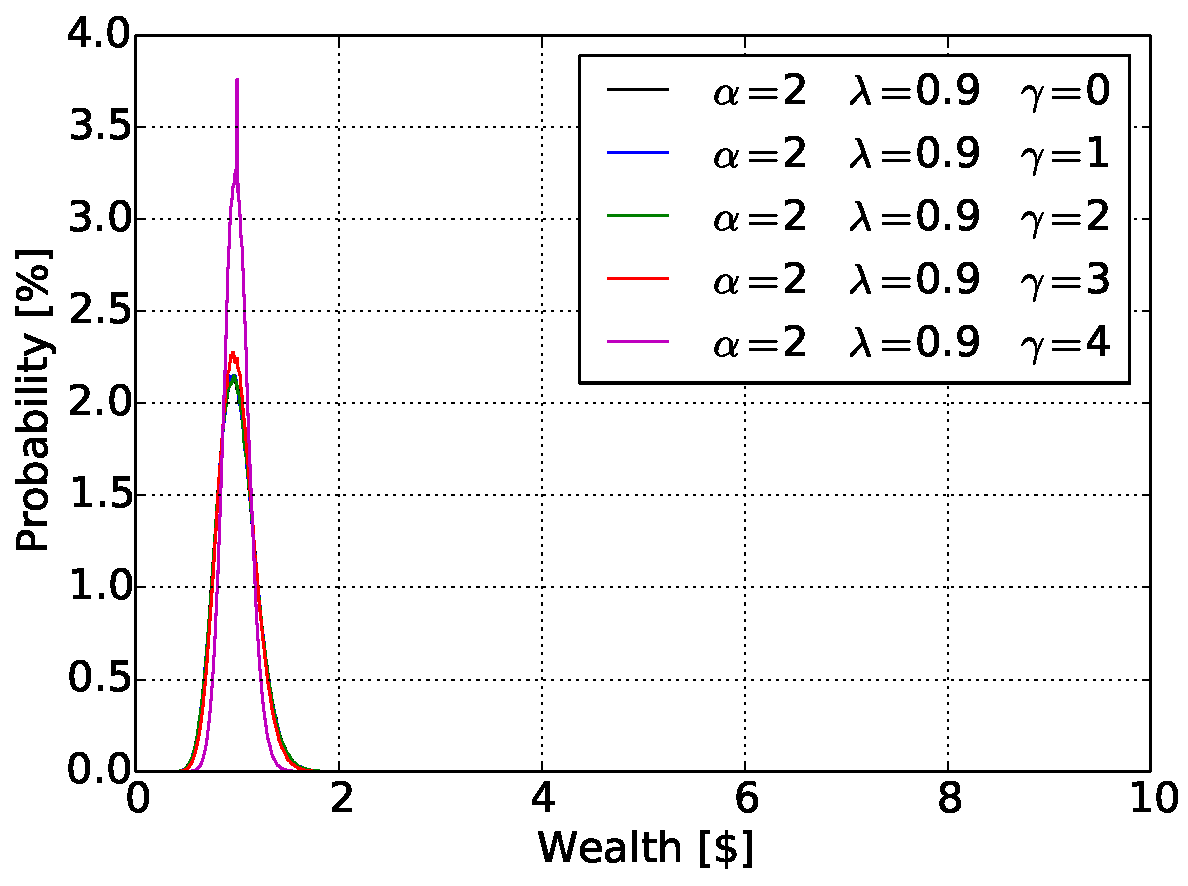
\includegraphics[width=\linewidth]{result/bilder/5e-2-90}
        \caption{}
    \end{subfigure}%
    ~ 
    \begin{subfigure}{0.5\textwidth}
        \centering
        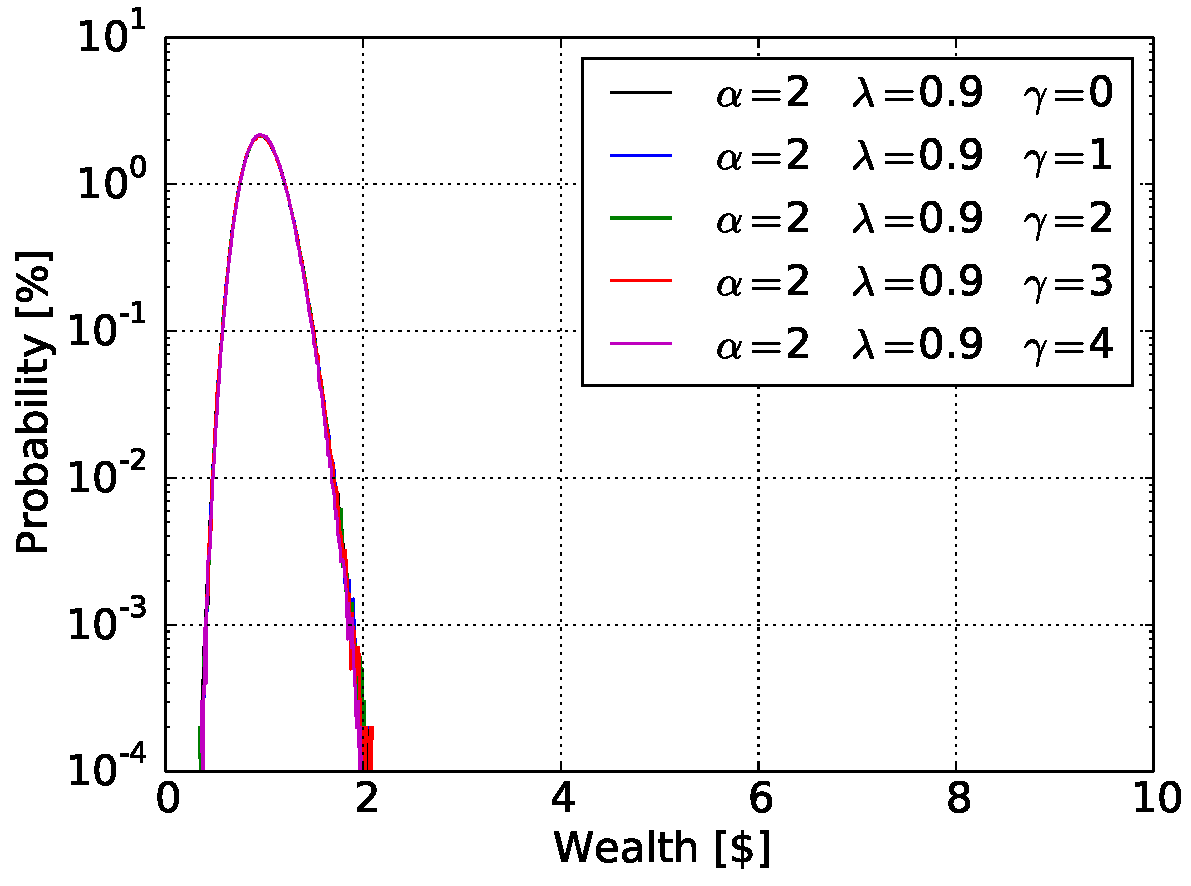
\includegraphics[width=\linewidth]{result/bilder/5e-2-90-log}
        \caption{}
    \end{subfigure}
    \caption{a) Shows how E behaves around $T_C$ b) Shows how |M| develops near $T_C$.}
    \label{fig:5e-2-90}
\end{figure}













